%!TEX root = main.tex
\setlength{\parskip}{\baselineskip} 
\section{Background}

\frame
{\frametitle{ Why care about mixtures? }
\begin{columns}
\column{0.5\textwidth}
\vspace{2ex} \\
    \begin{itemize}
        \item We are exposed to hundreds (thousands?) of chemicals at any single time point
        \item Traditionally, epi studies have focused on single-chemical analyses
        \begin{itemize}
            \item This does not represent reality
        \end{itemize}
        \item The {\color{matbluedark} combination} of exposures likely induces different responses 
    \end{itemize}
\column{0.5\textwidth}
\begin{center}
	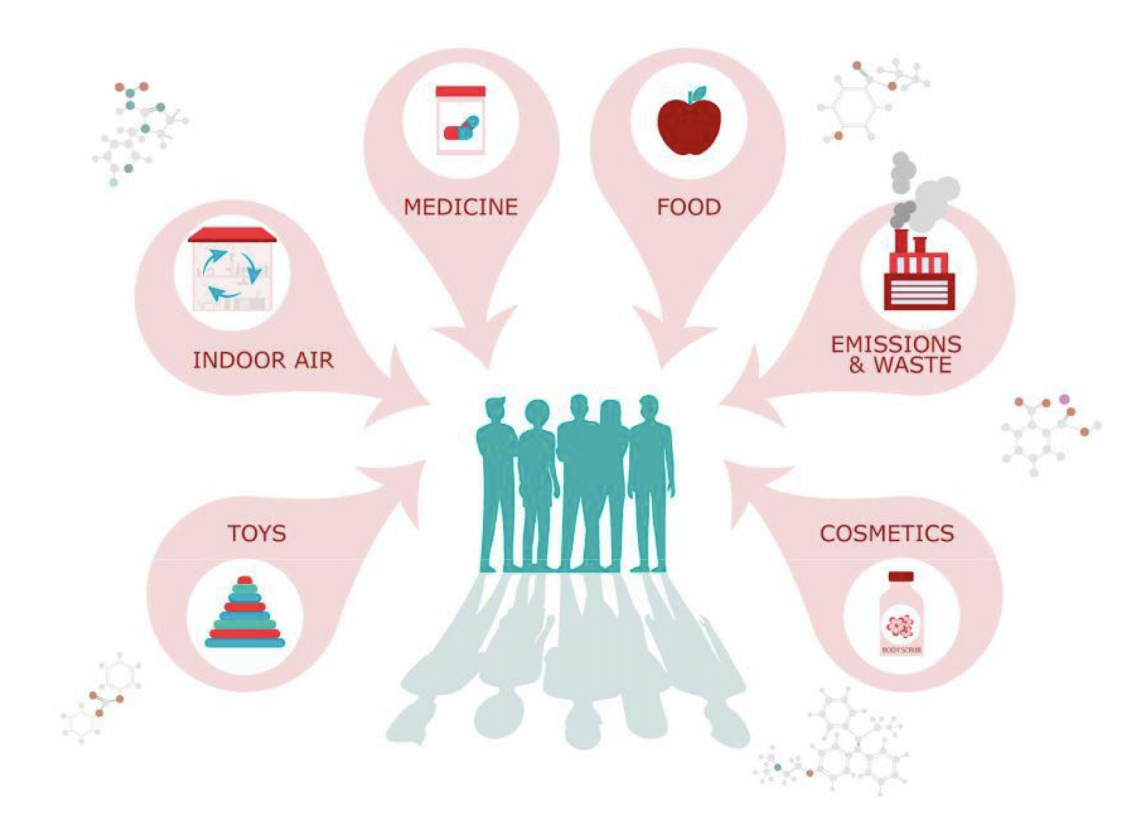
\includegraphics[scale=0.3]{figures/europa_image.png} \\
\raggedleft
	{\tiny\color{hgray}Image: ec.europa.eu via Yanelli N\'{u}\~{n}ez}
\end{center}
\end{columns}
}

\frame{\frametitle{ What is a mixture?}
    \begin{itemize}
        \item Actually, there is no strict definition \vspace{1ex}
        \item According to NIEHS ``{\tt a mixture must have at least three independent chemicals or chemical groups}'' \vspace{1ex}
        \item Generally, exposure to a mixture indicates exposure to {\color{matbluedark} multiple} ``stressors'' simultaneously \vspace{1ex}
        \begin{itemize}
            \item Chemical 
            \item Non-chemical (SES, diet, etc)
    \end{itemize}
    \end{itemize}
}

\frame{
\frametitle{Million dollar question}
    \begin{itemize}
	    \item The necessity to assess exposure to mixtures is now well-recognized
	    \item US EPA, NRC, and NIEHS all agree 
    \end{itemize}	
\pause
\vspace{5ex}
    \begin{tcolorbox}[colframe=matbluedark, colback=white]
	    \centering
	    {\color{matbluedark}How} can we represent the compexity of reality in a (single) statistical model? 	
    \end{tcolorbox}
}

\frame{\frametitle{ How do we deal with exposure to mixtures? }
    \begin{itemize}
        \item This is still a very open question
        \item Existing methods have limitations
        \item There have been several workshops held by EPA and NIEHS to address this issue
        \item The most recent NIEHS workshop (2015) concluded that 
        \begin{enumerate}
            \item Although some methods performed better than others, the presented estimated associations were still quite variable and not in agreement
            \item {\color{matbluedark}The choice of method should depend on the research question}
    \end{enumerate}
    \end{itemize}
}

\frame{\frametitle{Why do traditional methods fail?}
    \begin{itemize}
            \item Chemicals are often {\color{matbluedark}highly-correlated}
            \begin{itemize}
                \item This means that they cannot go in the same regression model
                \item[$\Rightarrow$] Large standard errors and unstable effect estimates
            \end{itemize}
            \item Requires more flexible models
            \begin{itemize}
                \item Group chemicals or assays
                \item Drop some chemicals
                \item Incorporate {\tt \color{matbluedark} machine learning techniques}
            \end{itemize}
    \end{itemize}
}

\frame{
\frametitle{Some considerations}\
    \begin{enumerate}
        \item No single method outperforms all others for all potential questions
        \item {\color{matbluedark} Interpretability}
        \item {\color{matbluedark} Robustness} (stable solutions)
        \item Computational scalability -- as $N$ and/or $p$ increase, some methods begin to fail
        \item Exploration vs. hypothesis testing
        \item Not a good idea to ``blindly'' use methods from other fields -- may need to adjust them first
    \end{enumerate}
}

\frame{
\frametitle{Potential questions in mixtures analyses}

    \begin{columns}
	\column{0.4\textwidth}
    	\begin{tcolorbox}[colframe=matbluedark, colback=white]
    		\centering
    		For mixtures analyses the selected method depends on the primary research question
	    \end{tcolorbox} 
	
	\column{0.6\textwidth}
	\vspace{2ex}
	    \begin{tikzpicture}[mindmap, grow cyclic,scale=0.8]
        	\begin{scope}[mindmap, concept color = white, text = matbluedark, 
        	level 1 concept/.append style = {level distance = 92, sibling angle = 72}]
        	\node [concept, text = matbluedark, scale = 0.55] at (0,0) (pattern) {{\huge Mixtures Research Questions}} [clockwise from = 15]
        	child [concept color = violet] {node [concept, text = white, scale = 0.7] (med) {{\large Overall Effect Estimation}}} 
        	child [concept color = green!50!black] {node [concept, text = white, scale = 0.7] (med) {{\large Pattern Recognition}}} 
        	child [concept color = blue] {node [concept, text = white, scale = 0.7] (med) {{\large Inter- actions}}} 
        	child [concept color = red] {node [concept, text = white, scale = 0.7] (med) {{\large {\it A priori} Defined Groups}}} 
        	child [concept color = orange] {node [concept, text = white, scale = 0.7] (med) {{\large Toxic Agent Identification}}} 
	;
	\end{scope}
	\end{tikzpicture}	
\end{columns}
}

\frame{
	\frametitle{Bird's-eye (over)view of existing mixtures methods}

	\raggedleft
	{\small\color{hgray}$^{\star}$Not an a exhaustive list of methods!!}	\\
	\vspace{-3ex}
	
	\centering
	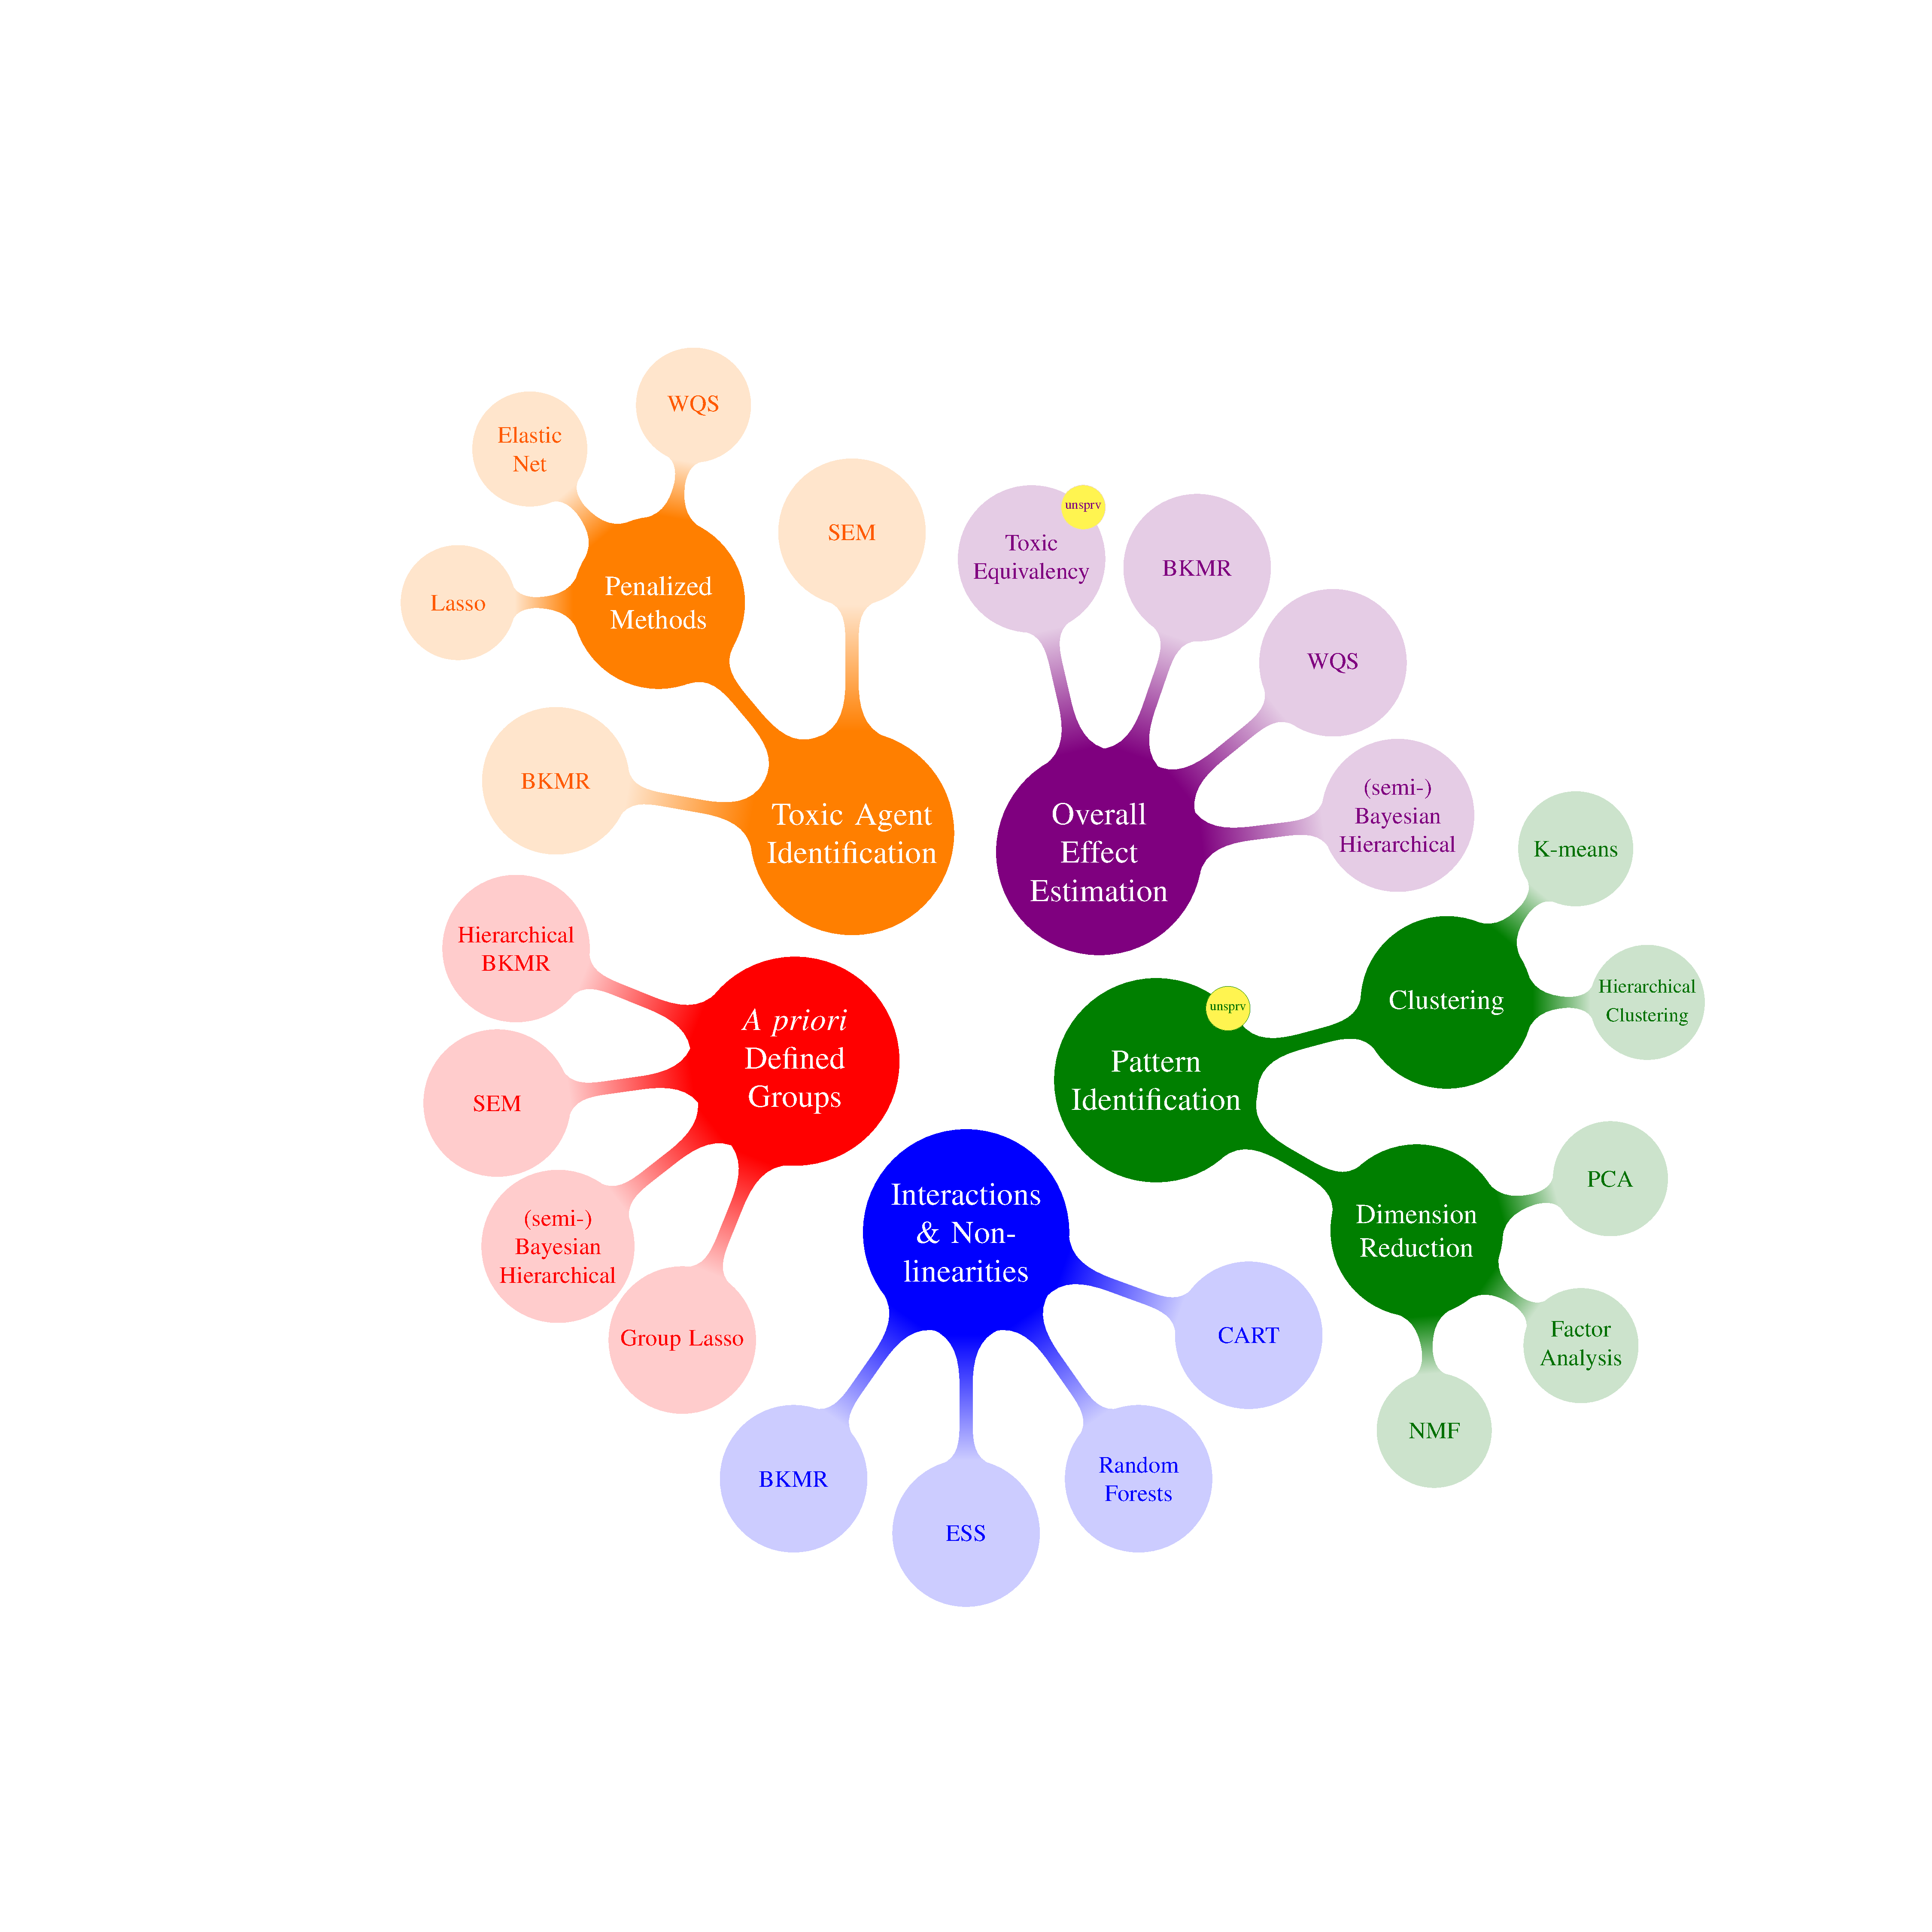
\includegraphics[scale=0.135]{figures/overview} \\
}

\frame{
	\frametitle{Comparing results across methods}
	\begin{itemize}
		\item Generally a good practice
		\begin{itemize}
			\item Especially if complementary methods 
			\item Sensitivity analyses to assess robustness of results  
		\end{itemize}
		\item If different methods address different questions, consistency in findings is welcome, but not expected
		\item If/when differences across methods are detected $\rightarrow$ keep in mind what the aim of each method is!
		\item Trying different methods and choosing the answer we like the best should {\it always} be avoided
		\begin{itemize}
			\item I.e., no cherry-picking!
		\end{itemize}
	\end{itemize}
}

\frame
{\frametitle{ Why care about mixtures? }
\begin{columns}
\column{0.5\textwidth}
\vspace{2ex} \\
    \begin{itemize}
        \item We are exposed to hundreds (thousands?) of chemicals at any single time point
        \item Traditionally, epi studies have focused on single-chemical analyses
        \begin{itemize}
            \item This does not represent reality
        \end{itemize}
        \item The {\color{matbluedark} combination} of exposures likely induces different responses 
    \end{itemize}
\column{0.5\textwidth}
\begin{center}
	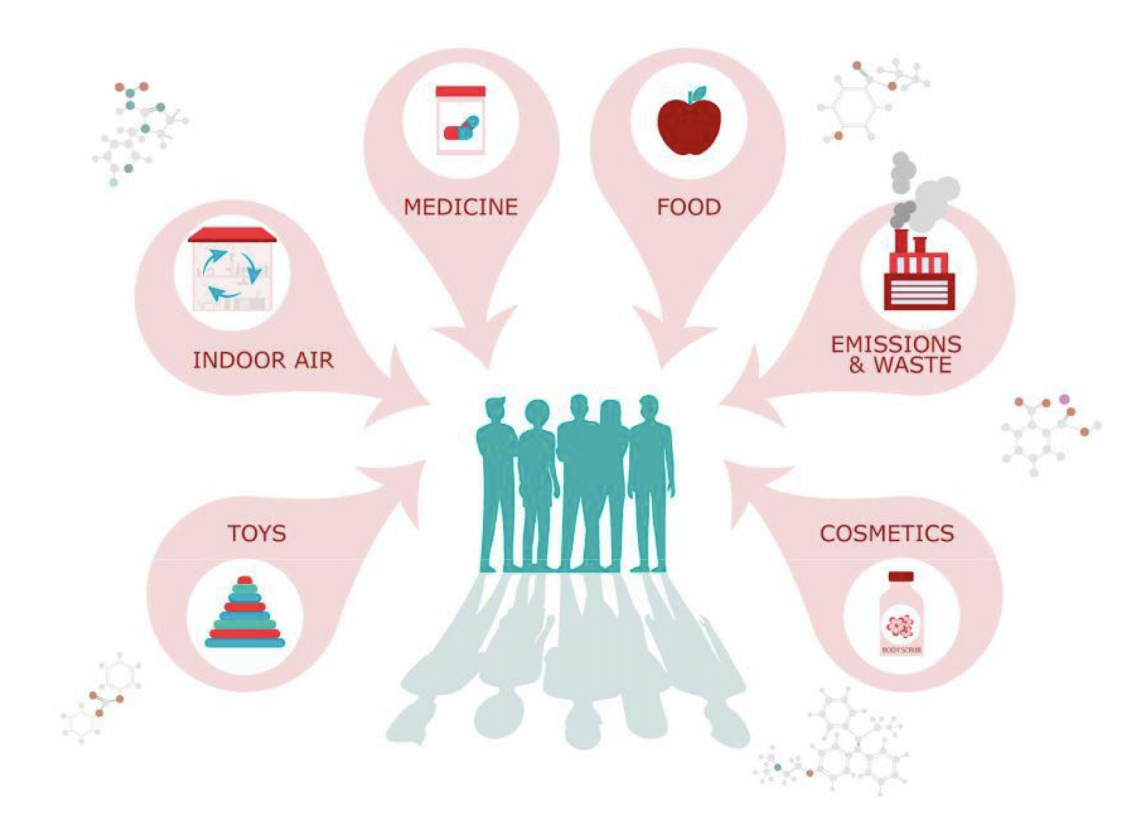
\includegraphics[scale=0.3]{figures/europa_image.png} \\
\raggedleft
	{\tiny\color{hgray}Image: ec.europa.eu via Yanelli N\'{u}\~{n}ez}
\end{center}
\end{columns}
}

\frame{
	\frametitle{Exposure pattern recognition}
	\begin{columns}
		\column{0.5\textwidth}
		\begin{itemize}
			\item Why should we care about identifying {\color{matbluedark}exposure patterns} to chemicals in a population?
			\begin{itemize}
				\item Sources
				\item Behaviors
			\end{itemize}
			\item If we link these patterns to (multiple) adverse health outcomes
			\begin{itemize}
				\item Efficient regulations
				\item Targeted interventions
			\end{itemize}
		\end{itemize}
		\column{0.6\textwidth}
			\vspace{2ex}
		 \begin{tikzpicture}[mindmap, grow cyclic,scale=0.8]
        	\begin{scope}[mindmap, concept color = white, text = matbluedark,
        	level 1 concept/.append style = {level distance = 92, sibling angle = 72}]
        	\node [concept, text = gray, scale = 0.55] at (0,0) (pattern) {{\huge Mixtures Research Questions}} [clockwise from = 15]
        	child [concept color = gray] {node [concept, text = white, scale = 0.7] (med) {{\large Overall Effect Estimation}}}
        	child [concept color = green!50!black] {node [concept, text = white, scale = 0.7] (med) {{\large Pattern Recognition}}} 
        	child [concept color = gray] {node [concept, text = white, scale = 0.7] (med) {{\large Inter- actions}}} 
        	child [concept color = gray] {node [concept, text = white, scale = 0.7] (med) {{\large {\it A priori} Defined Groups}}} 
        	child [concept color = gray] {node [concept, text = white, scale = 0.7] (med) {{\large Toxic Agent Identification}}} ;
		\end{scope}
		\end{tikzpicture}
\end{columns}
}

\frame{
	\frametitle{Some existing pattern recognition methods}

\centering\begin{tikzpicture}[mindmap, grow cyclic,scale=0.5]
  \begin{scope}[mindmap, concept color = green!50!black, text = green!40!black, 
  level 1 concept/.append style = {level distance = 150, sibling angle = 90},
  level 2 concept/.append style = {level distance = 115, sibling angle = 70}]
    \node [concept, text = white, scale = 0.55] at (0,0) (pattern) {{\LARGE Pattern Recognition}} [clockwise from = 315]
      child {node [concept, text = white, scale = .7] (med) {\large Clustering} [clockwise from=-35]
        child [concept color = green!45!black!20] {node [concept, scale = .7] {K-means}}
        child [concept color = green!45!black!20] {node [concept, scale = .7] {Hierarchical Clustering}}}
      child {node [concept, text = white, scale = .7] (gen) {\large Dimension Reduction}
        child [concept color = green!45!black!20] {node [concept, scale = .7] {PCA}}
        child [concept color = green!45!black!20] {node [concept, scale = .7] {Factor Analysis}}
        child [concept color = green!45!black!20] {node [concept, scale = .7] {NMF}}};
  \end{scope}
\end{tikzpicture}

\raggedleft
 	{\small\color{hgray}$^{\star}$Not an exhaustive list of methods!!}	\\
 	\vspace{1ex}
}

\frame{\frametitle{Why do traditional methods fail?}
    \begin{itemize}
            \item Chemicals are often {\color{matbluedark}highly-correlated}
            \begin{itemize}
                \item This means that they cannot go in the same regression model
                \item[$\Rightarrow$] Large standard errors and unstable effect estimates
            \end{itemize}
            \item Desire \textbf{\color{matbluedark}interpretable} results
            \item Require more flexible models
            \begin{itemize}
                \item Group chemicals or assays
                \item Identify underlying patterns
                \item Incorporate {\tt \color{matbluedark} machine learning techniques}
            \end{itemize}
    \end{itemize}
}

\frame{
	\frametitle{Existing exposure pattern recognition methods}
	\begin{columns}[c]
\column{0.6\textwidth}
\vspace{2ex}
\begin{tikzpicture}[mindmap, grow cyclic,scale=0.8]
\begin{scope}[mindmap, concept color = white, text = matbluedark,
        	level 1 concept/.append style = {level distance = 92, sibling angle = 72}]
\node [concept, text = matbluedark, scale = 0.55] at (0,0) (pattern) {{\huge Mixtures Research Questions}} [clockwise from = 15]
        	child [concept color = matbluelight] {node [concept, text = white, scale = 0.7] (med) {{\large Overall Effect Estimation}}}
        	child [concept color = matbluedark] {node [concept, text = white, scale = 0.7] (med) {{\large Pattern Recognition}}} 
        	child [concept color = matbluelight] {node [concept, text = white, scale = 0.7] (med) {{\large Inter- actions}}} 
        	child [concept color = matbluelight] {node [concept, text = white, scale = 0.7] (med) {{\large {\it A priori} Defined Groups}}} 
        	child [concept color = matbluelight] {node [concept, text = white, scale = 0.7] (med) {{\large Toxic Agent Identification}}} ;
\end{scope}
\end{tikzpicture}

    \column{0.5\textwidth}

        \begin{itemize}
         \item Choice of $k$ patterns subjective
         \item $+/-$ values not easily interpretable 
         \item Orthogonality constraint not realistic
         \item No measure of uncertainty
        \end{itemize}
\vspace{1ex}
\centering$\Longrightarrow$ Proposed solution: \\
\vspace{1ex}
{\tt\color{matbluedark}\textbf{Bayesian non-parametric non-negative matrix factorization}}

\end{columns}
}